\newpage
\section{Profilo utente}




\subsection{Pagamenti DA COMPLETARE}

Gli utenti sviluppatori possono consultare i propri dati finanziari, quali movimenti o saldo, nelle sezioni preposte del proprio profilo. La sezione Gestione conto mostra il saldo attuale e offre la possibilità di caricare il proprio saldo tramite funzionalità esterne (PayPal).

\label{Gestione conto}
\begin{figure}[H]
	\centering
	\fbox{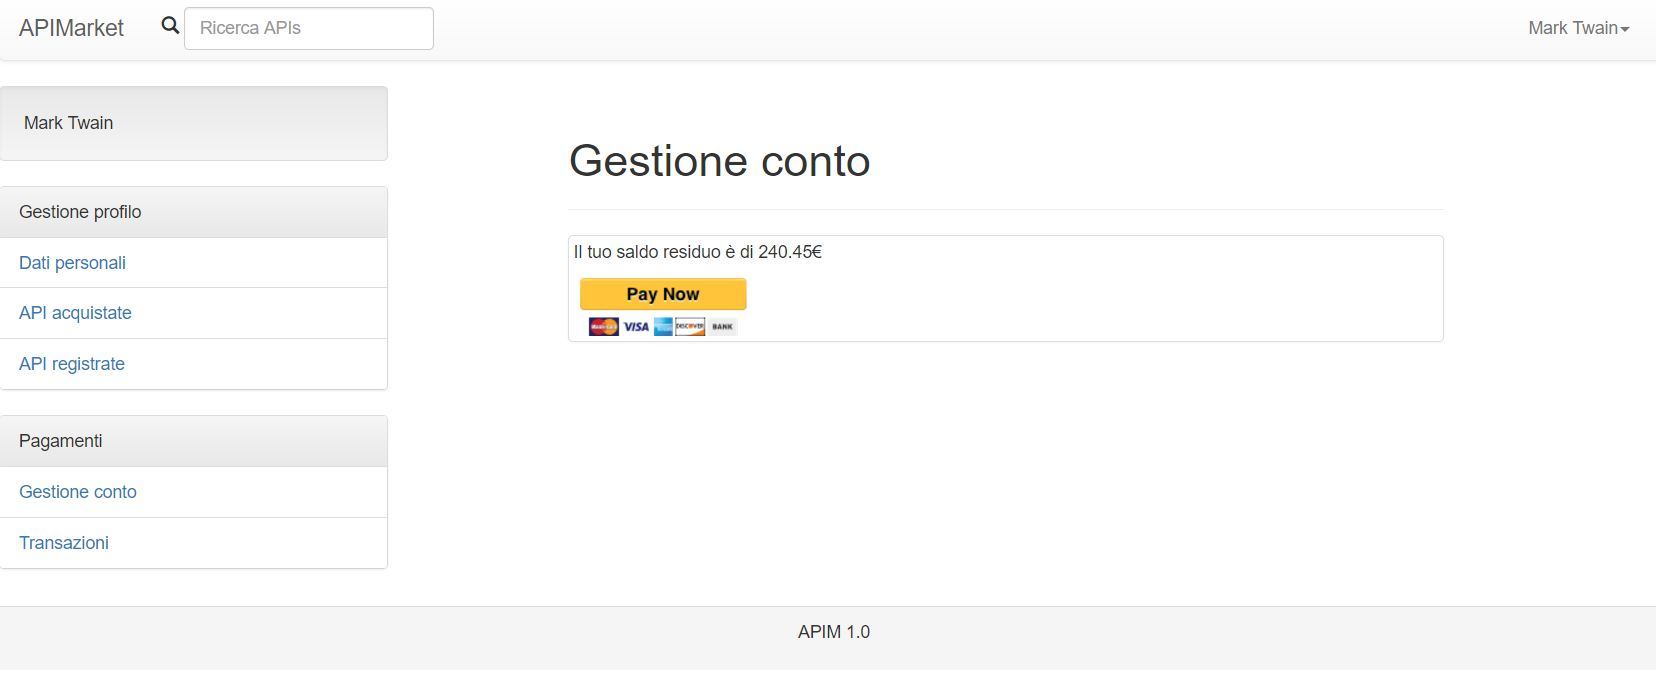
\includegraphics[scale=0.45]{img/APIM_gestioneConto.JPG}}
	\caption{Gestione conto}
\end{figure}

Nella voce transazioni, invece, è disponibile uno storico delle transazioni effettuate nell'API Market. Esse riguardano i servizi utilizzati e le relative chiamate, o gli addebiti per policy di altra tipologia. Lo storico contiene la designazione dell'API che è stata utilizzata, il costo, e la data. Esiste inoltre un ID univoco della transazione, per poter referenziare una particolare transazione con lo staff API Market.

\label{Transazioni}
\begin{figure}[H]
	\centering
	\fbox{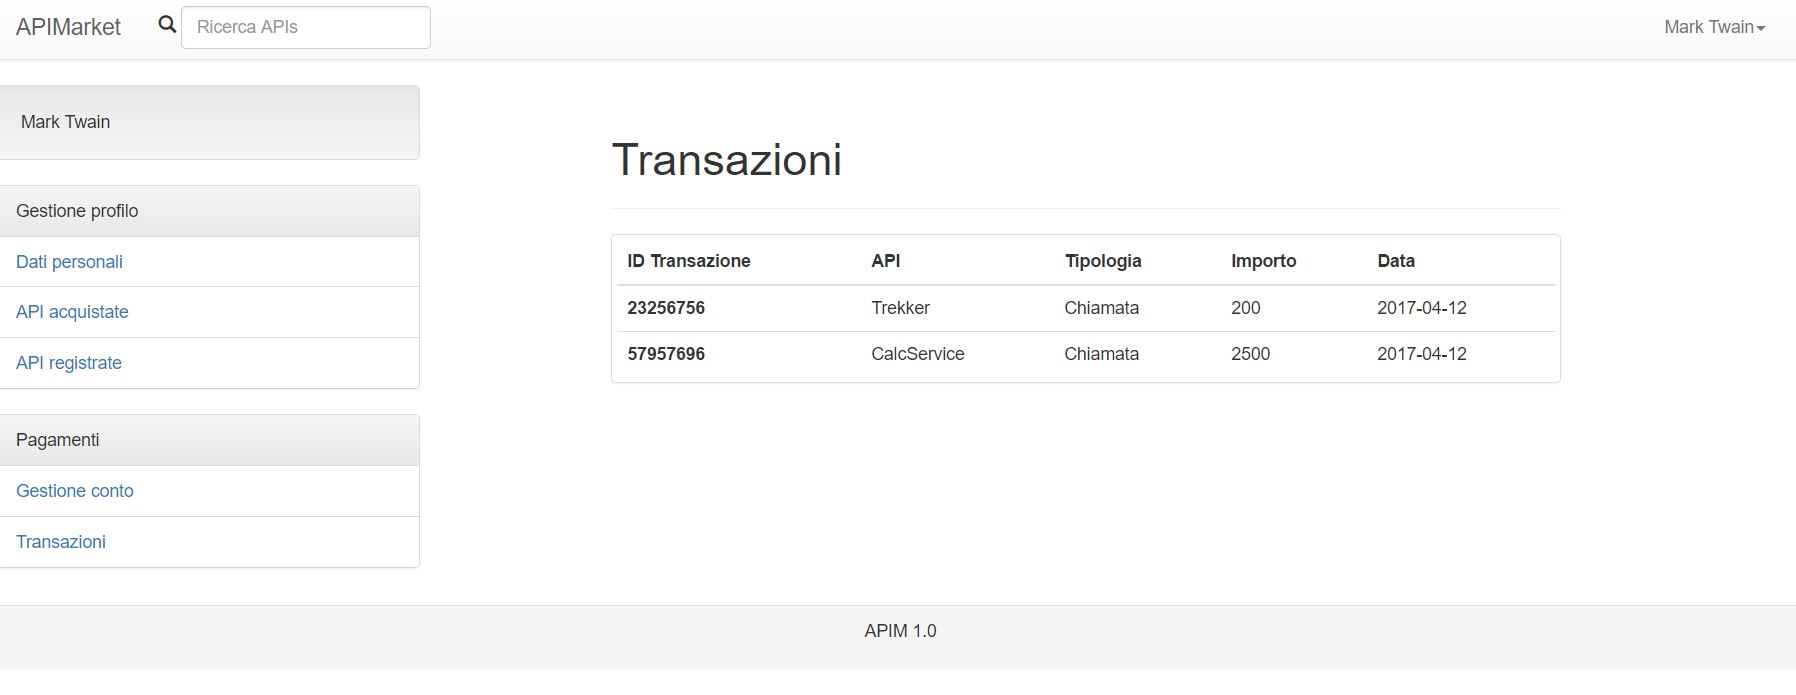
\includegraphics[scale=0.42]{img/APIM_transazioni.JPG}}
	\caption{Transazioni}
\end{figure}